% Copyright (c) 2014,2016 Casper Ti. Vector
% Public domain.

\chapter{PandaX-III项目介绍}
\label{chapter:1}
%\pkuthssffaq % 中文测试文字。

正如上文所说的,无中微子双Beta衰变事件是一种极其稀有的事件,既有实验已经给去它的半衰期$T^{0\nu}_1/2>1.07\times10^{26}$年,需要达成给出中微子质量顺序这一中期目标至少需要1吨量级的衰变元素。因而相应的实验难点便是以下四点:

\begin{enumerate}
    \item 顺利制造生产出吨级的可能发生NLDBD事件的放射性元素。
    \item 探测器具有极佳的能量分辨率和位置分辨率,能够准确的捕捉到NLDBD事件。
    \item 探测器本底噪声很低,在灵敏区域的背景事件应该小于0.1个每吨每年。
    \item 合适的数据处理方法来区分NLDBD事件以及和背景事件
\end{enumerate}

在诸多可以发生NLDBD事件的放射性元素中,PandaX-III选取了$^{136}$Xe作为目标,因为其在自然界中含量较为丰富,因而相对便宜。再有$^{136}$Xe作为衰变元素的同时也可以作为探测器的敏感气体,因而使用它可以制造出相当巨大的气体探测器。该元素NLDBD事件释放出的总能量为$Q_{\beta\beta}=2458keV$,这个能量相对较高,能够避免低能的背景辐射,但是在$Q_{\beta\beta}$附近也有来自$^{214}$Bi和$^{208}$Tl两种元素Gamma衰变的本底噪声。这两种元素作为$^{238}$U和$^{232}$Th衰变链中的中间元素广泛存在于自然界的各个角落中,因而也对使用$^{136}$Xe作为目标元素的NLDBD实验提出了巨大的挑战。

为了能够达到优秀的能量分辨率,Pandax-III计划建造5个200kg级别的高压气氙时间漂移室(time projection chamber, TPC)作为NLDBD的探测器,如图\ref{fig:detector}左所示。高压气体时间漂移室的技术在上个世纪90年代便已经成熟,相对与液体漂移时而言它能够提供更为优良的能量分辨率,如果使用直接读出电离电子数目的读取器件,高压气体TPC的分辨率能够接近达到液体的10倍。高压气体时间漂移室另外一个十分巨大的优势是能够较好的保留NLDBD事件的径迹,配合像素或者条状读出事件的径迹可以十分便捷的重建出,利用径迹信息可以极高效率的分辨出本地事件和NLDBD事件,从而能够几十倍的压低背景噪声。本文第\ref{section:3}章着重介绍了使用CNN分辨事件压低本地的方法。

\begin{figure}[tbp]
    \centering
    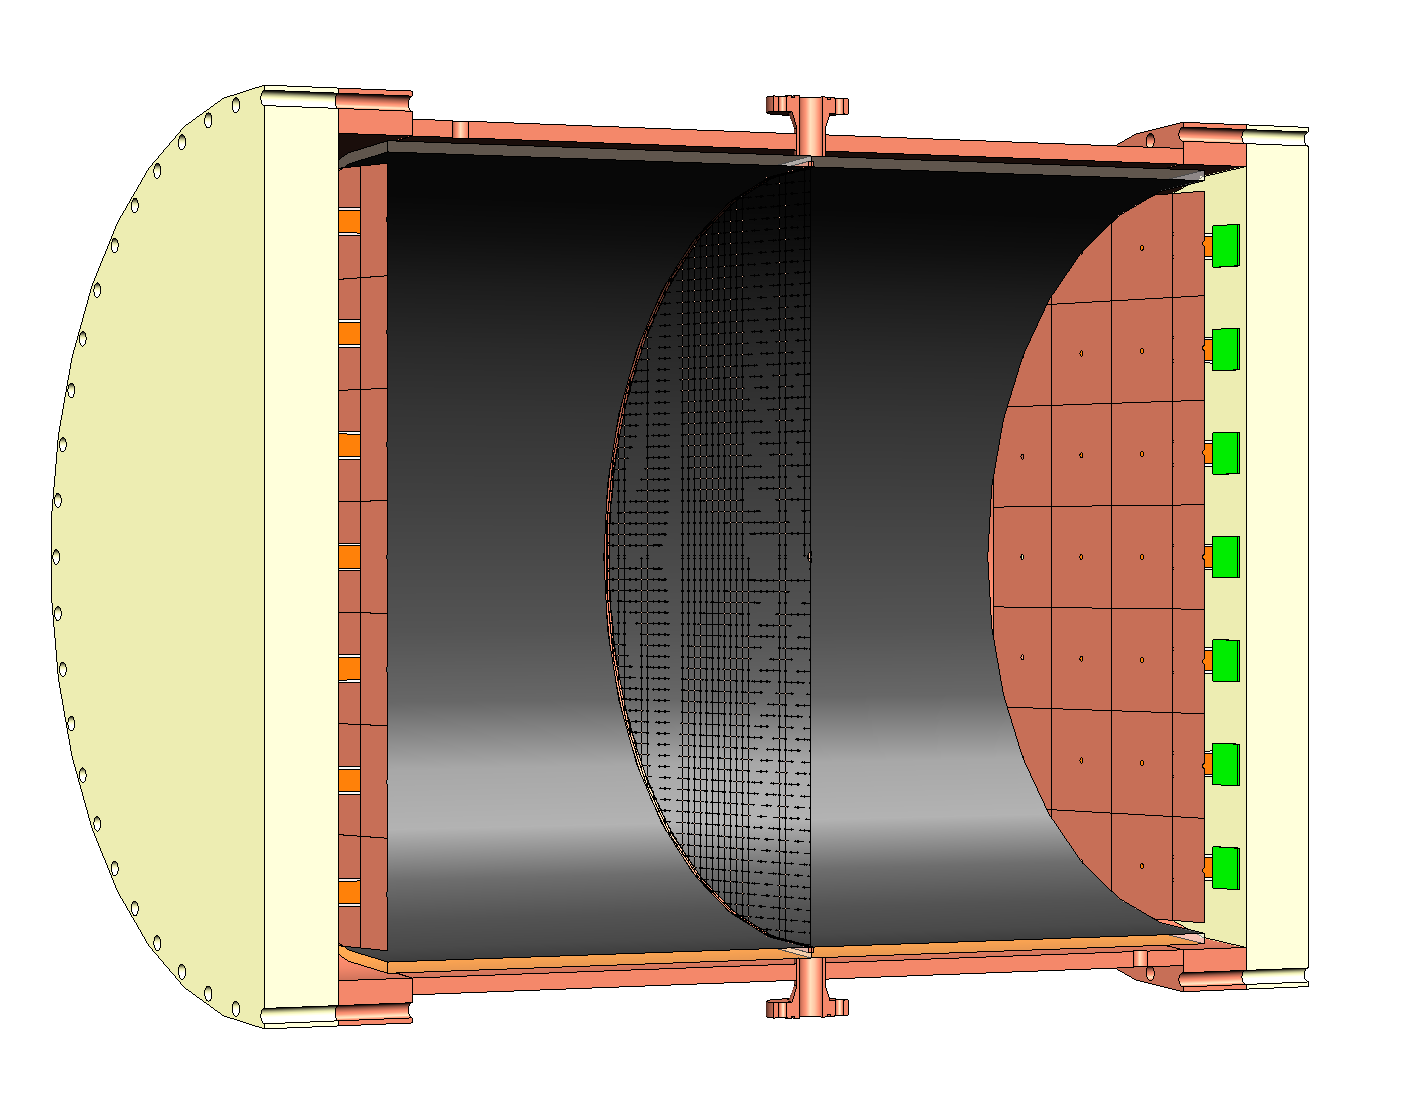
\includegraphics[width=0.4\columnwidth]{pic/fig1.png}
    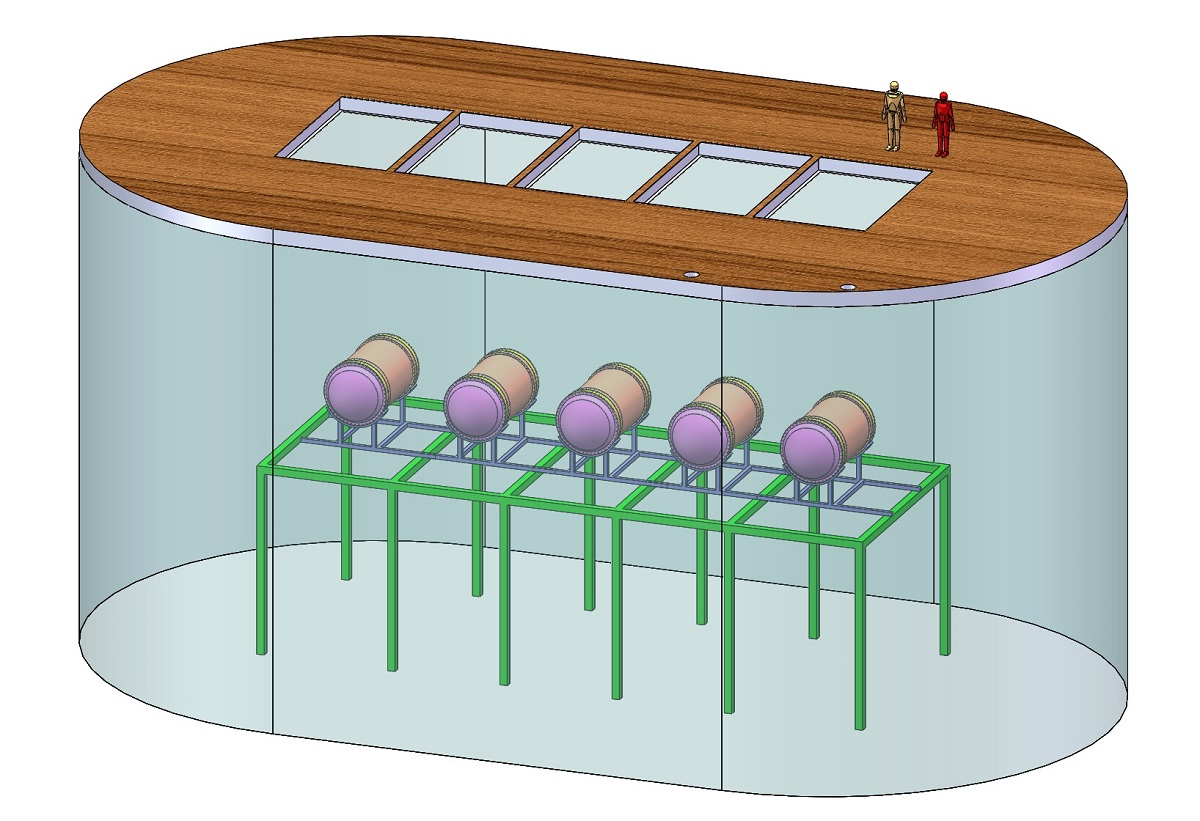
\includegraphics[width=0.4\columnwidth]{pic/fig2.jpg}
    \caption{左图:PandaX-III时间漂移室结构示意图。右图:5个TPC被放置在屏蔽水池示意图。}
    \label{fig:detector}
\end{figure}
    
    
\chapter{探测器背景事件模拟}
\chapter{利用CNN分辨NLDBD事件和背景事件}
\label{section:3}
% vim:ts=4:sw=4
